\documentclass[12pt]{article}

\usepackage[margin=1in]{geometry}
\usepackage{fancyhdr}
\usepackage{amsmath, amsfonts, amsthm, amssymb, mathtools}  % Some math symbols
\usepackage{color}
% \usepackage{sectsty}
\usepackage{tcolorbox}
\usepackage{amsfonts}
\usepackage{titletoc}
\usepackage{caption}
\usepackage[normalem]{ulem}
\usepackage{graphicx}


\usepackage{hyperref}
\hypersetup{
    colorlinks,
    citecolor=black,
    filecolor=black,
    linkcolor=black,
    urlcolor=black
}


\titlecontents{section}[0em]
{\smallskip}
{\thecontentslabel\enspace}
{\hspace*{-5.3em}}
{\hfill\contentspage}



%%%%%%%%%%%% SETUP %%%%%%%%%%%%

% name of the class
\newcommand{\classname}{CSE 371}
% name of the assignment
\newcommand{\assignmentname}{HW2}
% collaborators on assignment
\newcommand{\collaborators}{Cameron Jennings (ID: 2029631), Donovan Clay (ID: 2276005)}
\newcommand{\listcollaborators}{Collaborators: \collaborators}

\pagestyle{fancy}
\fancyhf{}
\setlength{\headheight}{13.59999pt}
\rhead{\thepage}
\lhead{\hyperref[beginning]{\classname \hspace{1em} \assignmentname}}

\usepackage{titlesec}
\titleformat{\subsection}{\normalfont\fontsize{12}{15}\bfseries}{\thesubsection}{1em}{}

\titleformat{\section}[block]
{\filcenter\large
\addtolength{\titlewidth}{2pc}%
\titleline*[c]{}%
\addvspace{6pt}%
}
{\thesection}{1em}{}
\titlespacing{\section}
{5pc}{*2}{*2}[5pc]


% \definecolor{WordSectionBlue}{RGB}{30, 90, 147}
% \allsectionsfont{\color{WordSectionBlue}}

%%%%%%%%%%%% FILE SPECIFIC IMPORTS %%%%%%%%%%%%

\usepackage{ragged2e}
\usepackage{tikz}

%%%%%%%%%%%%%%%%%%%%%%%%%%%%%%%%%%%%%%%%%%%%%%%

\renewcommand*{\thesection}{Question \arabic{section}.}
\renewcommand{\thesubsection}{(\alph{subsection})}

%%%%%%%%%%%% ENVIRONMENTS %%%%%%%%%%%%

\newenvironment{explanation}{\begin{tcolorbox}[colback=blue!2!white,colframe=blue!20!white]}{\end{tcolorbox}}

\newenvironment{subquestion}[1]{\subsection{#1}
\begin{tcolorbox}[colback=blue!2!white,colframe=blue!20!white]}{\end{tcolorbox}}

\newenvironment{sssq}[3]{\textbf{\thesubsubsection.\sssqARG{#1}} \hspace{0.5cm}
\begin{minipage}[t][\sssqARG{#2}][t]{14cm}
    \textbf{\sssqARG{#3}}
\end{minipage}
\begin{explanation}
}{\end{explanation}}

%%%%%%%%%%%% MY MACROS %%%%%%%%%%%%

\newcommand{\prob}{\mathbb{P}}
\newcommand{\expect}{\mathbb{E}}
\newcommand*\sssqARG{}
\newcommand{\bayes}{\textbf{Bayes' Theorem}}
\newcommand{\ltp}{\textbf{Law of Total Probability}}
\newcommand{\var}{\text{Var}}
\newcommand{\unif}{\sim \text{Unif}}
\newcommand{\expo}{\sim \text{Exponential}}
\newcommand{\caseif}{\text{if }}
\newcommand{\nlog}{\text{ln}}


%%%%%%%%%%%%%%%%%%%%%%%%%%%%%%%%%%%%%%
\begin{document}

    \setcounter{tocdepth}{1}
    \begin{center}\label{beginning}
        \tableofcontents 
    \end{center}

    \begin{center}
        \listcollaborators
    \end{center}

    % fix section heading font
    \titleformat{\section}{\normalfont\fontsize{17.28}{15}\bfseries\raggedright}{\thesection}{1em}{}
    \newpage
    \AddToHook{cmd/section/before}{\clearpage}

    % Question 1
    \section{}

        \begin{subquestion}{A binary multiplier that multiplies two 4-bit binary words}
            For each 4-bit word we are multiplying, there are 16 possible values it can have. So the number of combinations for the inputs is $16^2 = 256$. Then we know that for multiplying two 4-bit numbers, the ``worst case'' in terms of bits required to represent the output is 8-bits. So, we need \boxed{\text{256 words, 8 bits per word.}}
        \end{subquestion}    

        \begin{subquestion}{A 3-bit adder subtracter}
            For the 3-bit inputs there are $8^2 = 64$ possible combinations of the inputs. We will need an extra bit to specify if we want to add or subtract. The most output bits an operation would need is 4-bits because $111 + 111 = 1110$. So we will need \boxed{\text{128 words, 4-bits per word.}}
        \end{subquestion}

    \section{}
        \begin{subquestion}{How many 4Mi $\times$ 16 chips are needed to provide a total memory capacity of 64 Mi-bytes?}
            4Mi = $2^2$Mi = $2^2 \cdot 2^{20} = 2^{22}$.\\
            If the width of the chip is 16-bits = $2^4$ bits, then each chip has a capacity of $2^{22} \cdot 2^4 = 2^{26}$ bits. \\
            Our target for total memory capacity is 64 Mi-bytes = $2^6$ Mi-bytes = $2^6 \cdot 2^{20}$ bytes. = $2^6 \cdot 2^{20} \cdot 2^{3}$ bits = $2^{29}$ bits. So we will need $2^{29}/2^{26} = 2^{3}$ chips. \\
            \boxed{\text{8 4Mi $\times$ 16 chips}}
        \end{subquestion}

        \begin{subquestion}{How many address bits are needed for our larger, 64 Mi-byte-memory assuming the same word size as the individual chips?}
            Within one chip, we have $2^{22}$ words. We then need to decide between the 8 available chips. So we will have $2^{25}$ addresses. \\
            \boxed{\text{25 bits for $2^{25}$ addresses.}}

        \end{subquestion}

        \begin{subquestion}{How many of the address bits are connected to each RAM chip?}
            We will need to use 3 bits to determine which out of the 8 chips the data goes to. So we will have $25-3 = 22$ remaining bits for the address inside each chip.
        \end{subquestion}

        \begin{subquestion}{How many of the address bits must be decoded for the chip select?}
            There are 3 bits for the chip select. The size of the decoder is $3:8$ or $3 \times 8$.
        \end{subquestion}

    \section{}
        \begin{subquestion}{Show the resource utilization}
            Sign mag:
            \begin{center}
                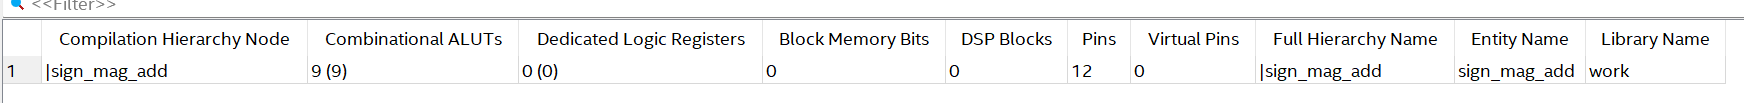
\includegraphics[scale = 0.5]{Images/resource 1.png}
            \end{center}
            Sync rom:
            \begin{center}
                \includegraphics[scale = 0.1]{Images/sync rom resources.jpg}
            \end{center}
        \end{subquestion}

    \section{}
        \begin{subquestion}{Complete the diagram below for an implementation of the $4\times 4$ register file.}
            \begin{center}
                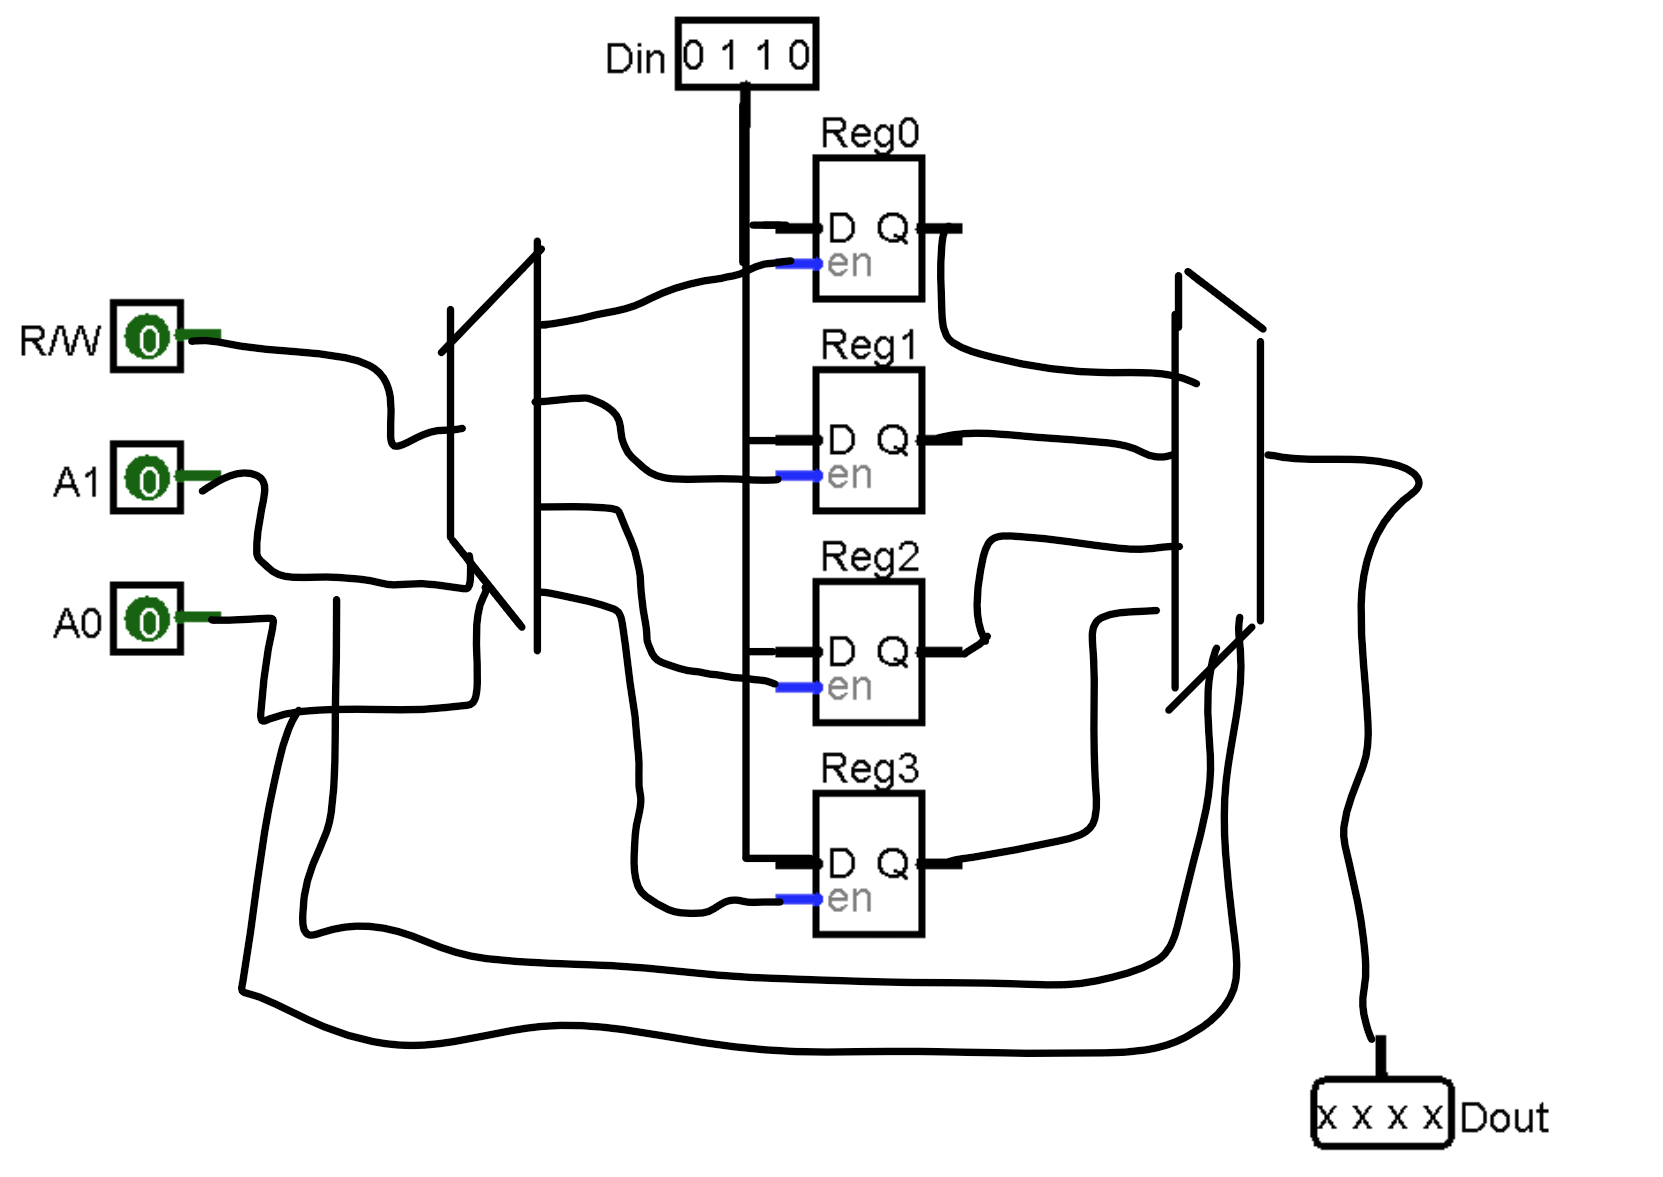
\includegraphics[scale = 0.5]{Images/4x4.png}
            \end{center}
        \end{subquestion}

        \begin{subquestion}{Construct a $8\times8$ memory diagram using the given $4\times 4$ as a building block.}
            \begin{center}
                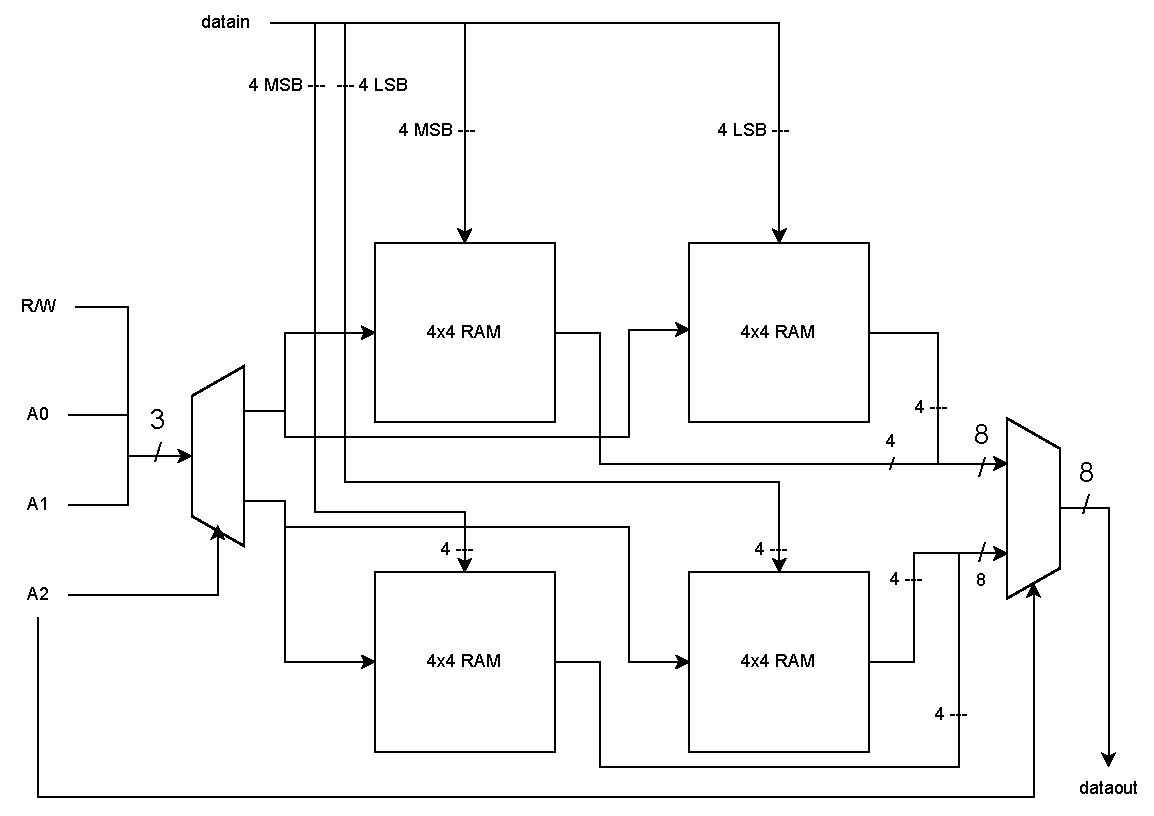
\includegraphics[scale=0.5]{Images/8x8 RAM diagram.pdf}
            \end{center}
        \end{subquestion}
        
        \section{Experience Report}
        We found this homework to be pretty simple and short. Problem 3 was definitely the most confusing and took the most time. 
        \begin{description}
            \item[Question 1:] 10 minutes
            \item[Question 2:] 10 minutes
            \item[Question 3:] 45 minutes
            \item[Question 4:] 20 minutes
        \end{description}        
\end{document}
